%   Filename    : chapter_4.tex 
\chapter{Research Methodology}
This chapter discusses the methodology used to develop the text and speech corpus for the Akeanon language, as well as building, training, and testing a model to generate initial results. The chapter is divided into five major parts: Data Collection, Text and Speech Corpus Development, Preprocessing, Validation, Building and Training A Model.

Figure~\ref{fig:flowchart} shows the general overview of the methodology for the development of an ASR system for the Akeanon language.

\begin{figure}[h!]
	\centering
	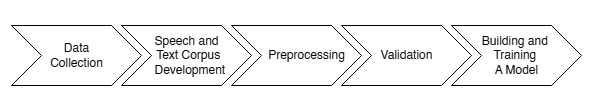
\includegraphics[width=\textwidth]{./figures/flowchart.png}
   \caption{Research Methodology}
	\label{fig:flowchart}
\end{figure}


\section{Data Collection}

\textbf{Collating Pre-existing Online Resources}

For the data collection, the researchers utilized existing online resources from the website, Bible.com. These resources include recordings and transcriptions of the Akeanon translations of the multiple books and chapters of the Bible. To retrieve the text transcriptions, the researchers developed a custom web scraper for Bible.com to automate the collection and compilation of Akeanon text for each book chapter. Meanwhile, the corresponding audio resources were manually recorded using Adobe Audition. These recordings serve as supplementary materials for the speech corpus.

\textbf{Gathering, Encoding, and Digitization of Non-Digital Resources}

The researchers gathered different Akeanon-based resources and text available at Kalibo Municipal library, to which include a dictionaries and thesaurus in Akeanon, songs, fables and tales, poems, and different collections of Akeanon text. The gathered resources were manually encoded and converted into digital format, storing it in a .txt file. For dictionaries and thesaurus, the materials were encoded and organized in a way that can be conveniently parsed for annotations. The Akeanon texts and literary pieces were encoded and stored in plain text for further analysis.

\textbf{Compiling Akeanon Words}

The researchers collected the Akeanon equivalent of the Swadesh 207 word-list, having the Aklanon to English Dictionary by \citeA{Reyes:1969}, A Thesaurus in Aklanon by \citeA{Pastrana:2012}, and Diksyunaryong Akeanon-English-Filipino by \citeA{Belayro:2015}, and multiple unpublished resources from \shortciteA{SIL:Malaynon, SIL:Bukidnon1, SIL:Bukidnon2} as references. All Akeanon words that can be found in all the collected and encoded resources were also considered, including the collated pre-existing online resources. In addition, words from different Akeanon dialects, namely Bukidnon, Buruangganon, Malaynon, and Nabasnon, were also compiled by the researchers through tapping native speakers for each dialect and built on the Swadesh list as a starting point. 

\textbf{Consonant and Vowel Inventories and Transcription}

After compiling the Akeanon word lists, the researchers had sought the assistance of Ms. Hazel Cipriano, a linguist who is also a native speaker of the language, to help create simplified  consonant and vowel inventories for the Akeanon language using the work of \shortciteA{Zorc:1995, Rentillo:2022} as reference for Akeanon phonology. Table~\ref{tab:simplified_consonant} and Table~\ref{tab:simplified_vowel} show the simplified consonant and vowel inventories. Instead of phonetic symbols, graphemes were used for the transcription. These simplified versions of the consonant and vowel inventories were used as reference when encoding the transcription of the words. Note that in this simplified version of the Akeanon consonant inventory, the glottal stop (\textipa{P}) is ignored for the transcription and some vowel phonemes were merged under one grapheme for the simplification of transcription of spoken Akeanon. The encoded transcription were used for building and training a model in Kaldi.

\begin{table}[H]
   \centering
   \caption{Simplified Consonant Inventory with Examples and Transcription} \vspace{0.25em}
   \label{tab:simplified_consonant}
   \renewcommand{\arraystretch}{1.2} % Adjust row height
   \setlength{\tabcolsep}{5pt} % Adjust column spacing
   \begin{tabular}{|c|c|c|c|}
       \hline
       \textbf{Consonant Symbol} & \textbf{Grapheme} & \textbf{Example Word} & \textbf{Transcription} \\ 
       \hline
       b & b & baeay & b a ea a y \\ \hline 
       d & d & daean & d a ea a n\\ \hline 
       g & g & gasto & g a s t o \\ \hline 
       h & h & hambae & h a m b a ea \\ \hline 
       k & k & kama & k a m a \\ \hline 
       l & l & lipat & l i p a t \\ \hline 
       m & m & mayad & m a y a d \\ \hline 
       n & n & nipa & n i p a \\ \hline 
       \textipa{N} & ng & ngipon & ng i p o n \\ \hline
       p & p & paea & p a ea a \\ \hline 
       \textfishhookr & r & relo & r e l o \\ \hline
       s & s & saea & s a ea a \\ \hline 
       t & t & tanan & t a n a n \\ \hline 
       \textturnmrleg & ea & eawas & ea a w a s \\ \hline
       j & y & yabi & y a b i \\ \hline 
       w & w & waea & w a ea a \\ \hline 
       (\textipa{dz}) & dz & dzai (slang) & dz a i \\ \hline 
       (\textipa{dZ}) & dy & madya & m a dy a \\ \hline
       (f) & f & Filipino & f i l i p i n o \\ \hline 
       (\textipa{S}) & sh & masyado & m a sh a d o \\ \hline
       (\textipa{ts}) & ts & matsa & m a ts a \\ \hline
       (\textipa{tS}) & ch & chamba & ch a m b a \\ \hline
       (v) & v & Visayas (name) & v i s a y a s \\ \hline  
       (z) & z & Zolina (name) & z o l i n a \\ 
       \hline
   \end{tabular}
\end{table}

\begin{table}[H]
   \centering
   \caption{Simplified Vowel Inventory with Examples and Transcription} \vspace{0.25em}
   \label{tab:simplified_vowel}
   \renewcommand{\arraystretch}{1.2} % Adjust row height
   \setlength{\tabcolsep}{5pt} % Adjust column spacing
   \begin{tabular}{|c|c|c|c|}
       \hline
       \textbf{Vowel} & \textbf{Grapheme} & \textbf{Example Word} & \textbf{Transcription} \\ 
       \hline
       a & a & aeang-aeang & a ea a ng a ea a ng \\ \hline
       e / (\textepsilon) & \textipa{e} & pwede & p w e d e \\ \hline
       i & i & ibog & \textipa{i b o g} \\ \hline
       o / (\textopeno) & \textipa{o} & oras & o r a s \\ \hline
       u & u & ugat & \textipa{u g a t} \\ 
       \hline
   \end{tabular}
\end{table}

\textbf{Ethical Considerations}

During the gathering of the different Akeanon-based resources and text, the researchers had sought consent from the respective authors and owners to use their works, in respect to intellectual property rights. See Appendix A for the screenshots of various authors and authors granting the researchers permission to use their works.

\section{Text and Speech Corpus Development}

\textbf{Storing}

After encoding and organizing the datasets across different sources accordingly, the data was extracted and stored in a central database for the entire word collection. To ensure uniformity among various data sources, a word was stored in the following format:
\\
\\
\\

\begin{lstlisting}[language=json, caption=Object structure for storing a word where each attribute represents a column, breaklines=true]
   {
   "word": "Hambaeon", // Akeanon word
   "attributes": {
      "transcription": "h a m b a ea o n", // Transcription
      "source": "Source of the word,
   }}
\end{lstlisting}

The compiled word list was stored in a .csv master file containing the following sheets: (a) Compiled Word List [MASTER]; (b) Transcription Guide; (c) Affixes; (d) Swadesh 207 Word List; and (e) SIL Word List. This ensures a more organized, accessible, and manageable database.

\textbf{Extraction}

For the extraction of words from the encoded text files, a Python script was created to parse each word from a specified text file. For most text files, the script finds all words and converts every word into lowercase to remove duplicates. Proper nouns were dealt with during the annotation and proofreading of the text corpus. However, there is a separate parser for the text files from Bible.com since they contain quite a number of proper nouns.

\textbf{Word and Text Selection for Speech Corpus}

For building the speech corpus, the researchers have prioritized words from the Swadesh 207 list for the voice recordings. The researchers also created a Python script that generated an additional 1000-word list to ensure phonemic coverage and lexical diversity beyond the Swadesh items. This script automatically filters out Swadesh entries from the master word list and selects 1,000 unique words that are phonemically diverse and suitable for recording. It ensures that all phonemes in the language were represented at least once and splits the final list into five balanced sets of 200 words each. Each set is exported into plain text files, both with and without their transcriptions, for ease of use during data collection and annotation. In the finalization of the sets, an excerpt from "Mga Suguilanon ni Tita Linda" and "Tales and Legends of Aklan (in Akeanon)" by \shortciteA{Belayro:Suguilanon, Belayro:Tales}, and an additional 30 sentences from "Mga Bueawanon Nga Hueobaton Sa Akeanon" by \shortciteA{Cichon:Bueawanon} were included to each set, to which all were unique.

\textbf{Voice Recording}

A total of 50 native speakers of Akeanon were gathered for the recording of the generated 1000-word list. The 1000-word list was divided into five sets, with each containing 200 words that were unique to that set. The speakers were gathered by batches and were made to randomly choose a set for them to read. For each set, there were 10 designated speakers for the recording. The researchers also collaborated with Aklan State University (ASU) - College of Teacher Education for the selection of speakers, with Dr. John Orbista as the primary contact. The speakers were of varying gender, and age to ensure diversity.

For the voice recordings of different dialects namely Bukidnon, Buruangganon, Malaynon, and Nabasnon, the researchers had tapped locals from the respective towns that speak the dialect. A total of 10 speakers for each dialect had their voices recorded. A modified set of the Swadesh 207-word list were provided for them, in respect of their spoken dialect. Table~\ref{tab:native_speakers} shows the categories of native speakers. 

\begin{table}[H]
   \centering
   \caption{Categories of Native Speakers} \vspace{0.25em}
   \label{tab:native_speakers}
   % Adjust row height and column padding
   \renewcommand{\arraystretch}{1.5} % Increase row height
   \setlength{\tabcolsep}{10pt} % Increase horizontal padding

\begin{tabular}{|c|p{2in}|} \hline
   \centering Category & Subcategories \\ \hline
   Sex & Male \\ 
   & Female \\ 
   \hline
   Age Group & 
   12-15 \\ 
   & 16-30 \\ 
   & 31-45 \\ 
   & 46-60 \\
   & 60+ \\ \hline
   Spoken Dialect & 
   Common Akeanon \\ 
   & Bukidnon \\ 
   & Buruangganon \\ 
   & Malaynon \\ 
   & Nabasnon \\ \hline
\end{tabular}
\end{table}

For the audio recordings, the microphone used was Shure SM58 (dynamic, cardiod pick-up pattern) with a Focusrite Scarlett 2i2 audio interface, having Adobe Audition 2021 as the recording software. For redundancy, an Elgato Wave:3 was also set up in case the main recording equipment failed. The audio files were named in the following convention: 

\texttt{\textless speaker\_number\textgreater\_\textless set\textgreater\_\textless gender\textgreater\_\textless age\textgreater\_\textless spoken\_dialect\textgreater}.wav

\textbf{Ethical Considerations}

At the beginning of their session for the voice recordings, participants were provided with a consent form, confidentiality agreement, and an information sheet containing information relevant to the study. This consent form served as a formal acknowledgment of the participant's voluntary involvement and understanding of the study's objectives, procedures, and potential risks. The form explained the purpose of the research, how the data will be used, and the steps taken to ensure confidentiality and anonymity. Participants were informed that they can withdraw from the study at any time without penalty. Additionally, the confidentiality agreement detailed the nature of the voice recordings and the storage of their data. Participants were made aware that their voices may be used for research analysis but will not be associated with their personal identities.

For minor participants, additional ethical measures were implemented. A separate Parental/Guardian Consent Form were provided, which outlined the same key information regarding the study, along with specific assurances about the protection of the minor’s privacy and confidentiality. This form sought explicit permission from the parent or guardian before the minor is allowed to participate. Parents or guardians were also given the opportunity to ask questions and were assured that their child’s participation was entirely voluntary. Furthermore, minors were asked to provide assent—a simplified acknowledgment that they understand the study and agree to participate. Both the parent/guardian consent and the minor's assent were required before participation can proceed. Throughout the study, the rights and welfare of minor participants were prioritized, and measures were taken to ensure their comfort and safety.

\section{Preprocessing}

\textbf{Annotation of the Text Corpus}

Each stored word contains the following attributes: phonetic transcription and source. These attributes serve as annotations for the processing of the dataset in the future. To automate the process of identifying the attributes and organizing them in one dataset, the researchers created a Python script that generates the grapheme transcription of the word.

Though more efficient, the researchers acknowledge that the automated process was prone to errors in generating the dataset, thus manual proofreading was still required, using "A Study of the Aklanon Dialect. Volume One: Grammar" by \shortciteA{deLaCruz:1968} as guide for spelling rules for Akeanon.

\textbf{Audio Cleanup and Preprocessing}

For preprocessing the audio files, Audacity was used for audio preprocessing. Noise reduction, bandwidth filters (high-pass: 200Hz, low pass: 18000 Hz), and a compressor were applied to the recorded audio and were then normalized to -0.1 dB. Each recording was then split into 10-second audio tracks, with each containing 10 word utterances for the word list. The recordings of the long-form text such as the excerpt and the 30 sentences was also split into 10 to 15-second audio tracks but contained word utterances between 10-25, depending on the speaker's reading pace. The tracks were renamed into the following convention:

\texttt{\textless dialect\textgreater\textless speaker\_id\textgreater\textless set\textgreater\textless text\_type\textgreater\_\textless sequence\_number\textgreater}.wav

Refer to Table~\ref{tab:namecoding} for the name coding of the 10-second audio tracks of the voice recordings.

\begin{table}[H]
   \centering
   \caption{Name Coding of the Split Audio Tracks} \vspace{0.25em}
   \label{tab:namecoding}
   
   \renewcommand{\arraystretch}{1.5} % Increase row height
   \setlength{\tabcolsep}{10pt} % Increase horizontal padding
   
   \begin{tabular}{|c|p{2in}|c|}
   \hline
   \textbf{Category} & \textbf{Subcategories} & \textbf{Coding} \\
   \hline
   Spoken Dialect & Common Akeanon & AK \\ 
   & Bukidnon & LI \\ 
   & Kalibonhon & KO \\ 
   & Buruangganon & RU \\ 
   & Malaynon & ML \\ 
   & Nabasnon & NS \\
   \hline
   Set & Swadesh & 0 \\ 
   & A & 1 \\ 
   & B & 2 \\ 
   & C & 3 \\ 
   & D & 4 \\  
   & E & 5 \\ 
   \hline
   Text Type & Word list & 00 \\ 
   & Short story & 01 \\ 
   & Sentences \& Idioms & 02 \\ 
   \hline
   \end{tabular}
\end{table}
   
Finally, the cleaned up audio tracks were exported in a WAV format stored in a folder named after the speaker number.

\section{Validation}

To validate the text and speech corpus, the researchers coordinated with native speakers and language experts to ensure the accuracy of spelling, grammar, and transcriptions. The transcription accuracy was further verified by comparing the transcriptions to the spoken content and ensuring consistency across the entire corpus. Dr. John E. Barrios from the University of the Philippines Visayas and Dr. Anthea R. Redison of the Center for West Visayan Studies, both native speakers of Akeanon, served as validators of the dataset.

\section{Building and Training a Model}

To generate initial results for the automatic speech recognition (ASR) system, a model was built, trained, and evaluated using the Kaldi toolkit on a selected subset of the speech corpus. A data split approach was employed, allocating nine recordings for training and one recording for testing. The training process progressed through the traditional Gaussian Mixture Model-Hidden Markov Model (GMM-HMM) pipeline. It began with a monophone model, which served as the foundation for aligning the training data. This was followed by a triphone model to capture contextual dependencies between phonemes, thus enhancing recognition accuracy.

To further improve performance, the triphone model was refined using Linear Discriminant Analysis (LDA) and Maximum Likelihood Linear Transformation (MLLT), which produced more discriminative feature representations. Finally, Speaker Adaptive Training (SAT) was applied through feature-space Maximum Likelihood Linear Regression (fMLLR), allowing the system to account for inter-speaker variability. This modeling progression follows the guidelines of \shortciteA{Chodroff:2018} and reflects best practices in traditional ASR development.

\textbf{Figure~\ref{fig:kaldi-pipeline}} illustrates the workflow of the ASR system development, highlighting the integration of data preparation, feature extraction, and model training stages. The diagram emphasizes the systematic approach taken to ensure a robust and efficient ASR system for the Akeanon language.

\begin{figure}[htbp]
   \centering
   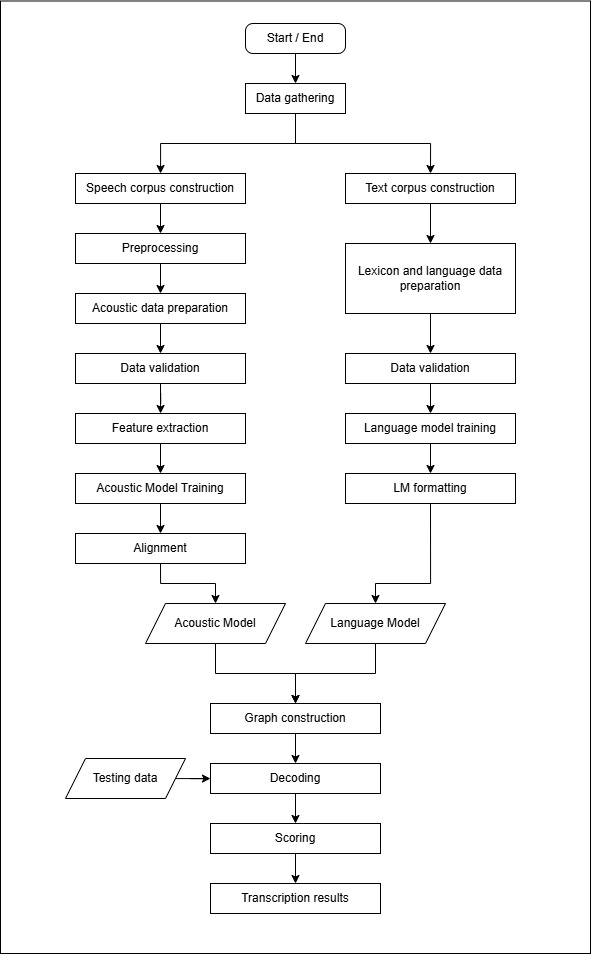
\includegraphics[width=0.8\textwidth, keepaspectratio]{./figures/kaldi-pipeline.jpg}
   \caption{Workflow of the ASR System Development}
   \label{fig:kaldi-pipeline}
\end{figure}

\subsection{Dataset Preparation Files}

\textbf{Acoustic Data Files}

The audio files were organized into a directory structure compatible with Kaldi's data preparation process. Each audio file was named according to the naming convention specified in the previous section, and the files were stored in a designated folder for each speaker. The audio files were then converted into a format suitable for Kaldi processing, ensuring that they were in the correct sample rate (16 kHz) and mono channel. For convenient mapping of the files in their respective sets and utterances they contain, an organized sheet file was prepared where relevant information was extracted by a custom script and the following files were generated as required by Kaldi data preparation process:

\begin{itemize}
       \item \textbf{wav.scp}: Maps each audio file identifier to its corresponding file path.
       \item \textbf{text}: Associates each utterance identifier with its transcription.
       \item \textbf{utt2spk}: Defines the mapping between each utterance and its corresponding speaker.
       \item \textbf{spk2gender}: Specifies the gender of each speaker.
\end{itemize}

These files collectively enable Kaldi to organize and process the audio data efficiently. The \texttt{wav.scp} file links audio files to their identifiers, while the \texttt{text} file provides the corresponding transcriptions. The \texttt{utt2spk} file ensures that each utterance is associated with the correct speaker, and the \texttt{spk2gender} file adds speaker gender information, which can be used for analysis or model adaptation.

The expected file formats are shown below:

\begin{table}[H]
\centering
\renewcommand{\arraystretch}{1.3}
\setlength{\tabcolsep}{10pt}
\caption{File Format Specifications for Dataset Preparation}
\label{tab:fileformats}
\begin{tabular}{|l|l|}
\hline
\textbf{File} & \textbf{Format} \\
\hline
\texttt{wav.scp} & \texttt{<file\_id> <path\_to\_file>} \\
\texttt{text} & \texttt{<utterance\_id> word1 word2 word3 ...} \\
\texttt{utt2spk} & \texttt{<utterance\_id> <speaker\_id>} \\
\texttt{spk2gender} & \texttt{<speaker\_id> <gender>} \\
\hline
\end{tabular}
\end{table}

\textbf{Lexicon and Language Data Files}

In preparation for the language modeling, the researchers created several files that define the pronunciation lexicon, silence phones, and non-silence phones used in the ASR system. Silence phones represent pauses or breaks in speech, which are crucial for distinguishing between words and phrases, while non-silence phones represent the actual speech sounds. The lexicon file was generated by a custom script where it maps all the words used in the speech data from the constructed text corpus and their corresponding transcriptions. These files were essential for building the language model and ensuring that the ASR system could accurately recognize and decode spoken Akeanon words. The following files were created:

\begin{itemize}
    \item \textbf{lexicon.txt}: Lists all words used in the project dictionary along with their corresponding phonemic transcriptions. Silence phones are also included.
    \item \textbf{nonsilence\_phones.txt}: Contains all non-silence phones used in the project.
    \item \textbf{silence\_phones.txt} and \textbf{optional\_silence.txt}: Specify the set of silence phones.
\end{itemize}

\vspace{1em}

The expected formats for the language data files are shown below:

\begin{table}[H]
\centering
\renewcommand{\arraystretch}{1.3}
\setlength{\tabcolsep}{10pt}
\caption{File Format Specifications for Language Modeling}
\label{tab:languageformats}
\begin{tabular}{|l|l|}
\hline
\textbf{File} & \textbf{Format} \\
\hline
\texttt{lexicon.txt} & \texttt{<word> <phone1> <phone2> ...} \\
\texttt{nonsilence\_phones.txt} & \texttt{<phone>} (one per line) \\
\texttt{silence\_phones.txt} & \texttt{<silence\_phone>} (one per line) \\
\texttt{optional\_silence.txt} & \texttt{<silence\_phone>} (single line) \\
\hline
\end{tabular}
\end{table}

\vspace{1em}

Data verification and cleanup were performed using built-in functionalities in Kaldi. The toolkit provides scripts to check the consistency and integrity of data directories, ensuring that all required files are present and correctly formatted. Utilities such as \texttt{utils/fix\_data\_dir.sh} and \texttt{utils/validate\_data\_dir.sh} were used to automatically detect and resolve common issues, such as missing or mismatched entries, duplicate utterances, or incorrect file references. This step was essential to prevent errors during feature extraction, model training, and decoding, and to maintain the reliability of the experimental results.

\subsection{Language Modeling}
For language modeling, a unigram count file was generated using a custom script based on the training set transcriptions. This file listed each unique word from the training corpus alongside its frequency of occurrence, representing the basic statistical distribution of word usage. The goal was to generate a simple unigram language model suitable for integration into the ASR decoding pipeline.

However, the unigram model has significant limitations due to its lack of context. It assumes that each word is generated independently of the words that precede or follow it, which can lead to inaccuracies in predicting word sequences, especially in languages with complex grammatical structures. For example, it cannot capture dependencies between words, such as subject-verb agreement or collocations. In contrast, more complex models like bigram or trigram models consider the relationships between consecutive words, providing better contextual understanding at the cost of increased computational complexity and data requirements. Despite its simplicity, the unigram model serves as a useful baseline for evaluating the performance of the acoustic model without introducing additional dependencies. A snippet of the unigram file is shown in Table~\ref{tab:unigram}.

\begin{table}[h]
\centering
\caption{Format of Unigram Count File}
\label{tab:unigram}
\begin{tabular}{ll}
\toprule
\textbf{Word} & \textbf{Frequency} \\
\midrule
RO            & 310 \\
IT            & 211  \\
NGA           & 173  \\
...           & ... \\
\bottomrule
\end{tabular}
\end{table}

\subsection{Phoneme Frequency Analysis}
To analyze the phoneme frequency in the Akeanon language, a Python script was developed to parse the phonetic transcriptions of the words in the compiled word list. The script counted the occurrences of each phoneme across all transcriptions, providing insights into the phonemic distribution within the language. The results of this analysis were stored in a text file, which contained two columns: the phoneme and its corresponding frequency count. This data was essential for understanding the phonetic characteristics of Akeanon and for guiding the design of the acoustic model. A snippet of the phoneme frequency count file is shown in Table~\ref{tab:phoneme}.

\begin{table}[h]
\centering
\caption{Format of Phoneme Frequency Count File}
\label{tab:phoneme}
\begin{tabular}{ll}
\toprule
\textbf{Word} & \textbf{Frequency} \\
\midrule
a            & 100 \\
b            & 99  \\
e            & 98  \\
...           & ... \\
\bottomrule
\end{tabular}
\end{table}

\subsection{Acoustic Model Training}
For acoustic model training, the Kaldi toolkit was used to build a series of progressively refined models based on the prepared speech corpus. The training process followed the standard Gaussian Mixture Model–Hidden Markov Model (GMM-HMM) pipeline, beginning with a monophone model and culminating in a speaker-adaptive triphone model. Each stage of model development relied on alignments generated from the previous model, allowing successive models to be trained on increasingly accurate supervision.

The pipeline was structured as follows:

\begin{enumerate}
    \item \textbf{Monophone Training}: The process began by training a basic monophone model, which treats each phoneme independently of its context. Although simple, this model provided the necessary initial alignments between audio frames and phonetic units, which served as a foundation for more advanced models.

    \item \textbf{Triphone Training with Delta Features (tri1)}: Using the alignments from the monophone model, a context-dependent triphone model was trained. This model incorporated delta and delta-delta features to capture first and second-order temporal dynamics in the audio signal, improving the model’s sensitivity to changes in speech patterns.

    \item \textbf{Triphone Training with LDA+MLLT (tri2a)}: To further enhance discriminability, Linear Discriminant Analysis (LDA) was used to project features into a lower-dimensional space that maximized phonetic class separability. Maximum Likelihood Linear Transform (MLLT) was then applied to refine the feature space through global transformations, resulting in more robust acoustic modeling.

    \item \textbf{Speaker Adaptive Training (SAT, tri3a)}: Finally, Speaker Adaptive Training was performed using feature-space Maximum Likelihood Linear Regression (fMLLR). This approach adapts features at the speaker level, allowing the model to account for inter-speaker variability and improve recognition accuracy in speaker-diverse conditions.
\end{enumerate}
Each training stage involved model estimation followed by forced alignment using Kaldi’s built-in scripts. The final SAT-enhanced triphone model (tri3a) was then integrated with the pronunciation lexicon and language model to perform decoding and generate automatic speech recognition (ASR) outputs. During training, the number of Gaussian mixtures (leaves) was controlled to range between approximately 2,500 and 15,000, depending on the model complexity and training stage. This range balances model expressiveness with the available amount of training data, ensuring stable and effective acoustic modeling without overfitting.

These settings follow common practices in GMM-HMM training using Kaldi, where the mixture size is gradually increased to better capture acoustic variability.

The GMM-HMM pipeline was used exclusively in this study due to its reliability, interpretability, and compatibility with low-resource settings. Deep learning–based acoustic models, such as DNN-HMM or end-to-end architectures, typically require larger datasets and more computational resources for effective training. In contrast, GMM-HMM models can be trained effectively on smaller corpora and provide a sound foundation for understanding core ASR concepts. Moreover, the GMM-HMM framework is well-supported by Kaldi’s modular architecture and remains a common baseline in both academic and applied ASR research.

\subsection{Decoding Graph Construction}
The unigram model was then compiled into the decoding graph alongside the acoustic and lexical models using Kaldi’s graph-building utilities. This process involved integrating the pronunciation lexicon, the set of phones, and the unigram language model into a finite-state transducer (FST) decoding graph. The resulting graph provided the ASR system with a structured representation of all possible word sequences, constrained by the lexicon and language model probabilities.

During decoding, the ASR system used this graph to search for the most likely word sequence given the observed acoustic features. The unigram language model contributed by assigning probabilities to individual words based on their frequency in the training corpus, while the acoustic model evaluated the likelihood of the audio features for each hypothesized word sequence. Although the unigram model does not capture word-to-word dependencies, its integration ensured that the system favored more frequent words and provided a baseline for evaluating the effectiveness of the acoustic and lexical modeling.

This approach allowed for a modular and extensible decoding pipeline, where more complex language models (such as bigram or trigram models) could later be substituted to improve recognition accuracy as more data became available.

\subsection{Decoding and Evaluation}
The decoding process was performed using Kaldi’s decoding scripts, which utilized the trained acoustic model, the pronunciation lexicon, and the unigram language model to transcribe the audio recordings. The decoding was executed on a test set of audio files, which were not used during the training phase, to evaluate the model's performance on unseen data. The decoding process involved extracting features from the audio files, aligning them with the phonetic transcriptions, and generating word hypotheses based on the acoustic and language models. The decoding results were stored in a text file, which contained the recognized words along with their corresponding utterance. This file served as the output of the ASR system, providing a transcription of the spoken Akeanon words from the audio recordings.

\subsection{Evaluation Metrics}
To assess the performance of the ASR system, the primary metric used was Word Error Rate (WER), which quantifies the percentage of words that were incorrectly recognized by the system. WER is calculated as follows:

\[
\text{WER} = \frac{S + D + I}{N} \times 100\%
\]

where \( S \) is the number of substitutions, \( D \) is the number of deletions, \( I \) is the number of insertions, and \( N \) is the total number of words in the reference transcription.

Kaldi provides built-in tools to compute WER by comparing the system’s output with the ground truth transcriptions. The evaluation results were analyzed to identify common recognition errors and to guide further improvements in the model and data preparation process.

The decoding and evaluation steps completed the ASR system pipeline, enabling the researchers to objectively measure the system’s accuracy and identify areas for refinement. The results from this stage provided a baseline for future enhancements, such as incorporating more advanced language models or expanding the training dataset.